%Standard Header
\documentclass[11pt,a4paper,toc=listof,toc=bibliography]{scrartcl}
\usepackage[utf8]{inputenc}
\usepackage[ngerman]{babel}
\usepackage[T1]{fontenc}
\usepackage{amsmath}
\usepackage{amsfonts}
\usepackage{amssymb}
\usepackage[pdftex]{graphicx}

%\usepackage{epstopdf}                            %import .eps (from MATLAB)
\usepackage{geometry}
\usepackage{multirow}
\usepackage{pdfpages}                            %import pdf
\usepackage{textcomp}                            %degree celsius etc
\usepackage{gensymb}
\usepackage[hidelinks]{hyperref}                 %hidelinks removes red boxes from pdf
\usepackage[style=german, german=quotes]{csquotes}
\usepackage[backend=biber, style=numeric, citestyle=numeric, sorting=none]{biblatex}
\usepackage{float}

\usepackage[all,defaultlines=2]{nowidow}		%prevent Witwen and Schusterjungen
\usepackage{microtype}

\usepackage{color}
\usepackage{listings}                            %einbinden von Sourcecode

%\usepackage{chemfig}
\usepackage{upgreek}
\usepackage{chemmacros}
\usepackage{chemformula}

\addbibresource{../DATA/bibresource.bib}        %Standardpfad für .bib Datei des Projektes

\usepackage{lmodern}

%\KOMAoption{DIV}{12}

%%%% alte Definition:
%% \DeclareMathSymbol{,}{\mathpunct}{letters}{"3B}
%%%% neue Definition:
%%\DeclareMathSymbol{,}{\mathord}{letters}{"3B}       %removes space in mathmode
\DeclareMathSymbol{*}{\mathbin}{symbols}{"01}

\newcommand{\mlab}{MATLAB}
%\renewcommand{\figurename}{Abb.}    %for article/report and non KOMA-Classes
\renewcaptionname{ngerman}{\figurename}{Abb.}

\setlength{\parindent}{0pt}          %keine Einschübe bei neuem Absatz

\addtokomafont{disposition}{\rmfamily} % serifes in headings

%SI-Units and correct spacing according to ISO-31
\usepackage[range-phrase = \ldots~]{siunitx}
\sisetup{locale=DE}
\sisetup{inter-unit-product=\ensuremath{{}*{}}}
\sisetup{per-mode=symbol}
%Listings environment for sourcecode
%\renewcommand{\lstlistlistingname}{Sourcecode}     %name in listof"sourcecode"
%\renewcommand{\lstlistingname}{Code}            %captionPreName

\lstset{breaklines}
\lstset{numbers=left}
\lstset{frame=single}
%\lstset{language=Matlab}
\lstset{showstringspaces=false}
\lstset{ %
	backgroundcolor=\color{white},   % choose the background color
	basicstyle=\footnotesize,        % size of fonts used for the code
	breaklines=true,                 % automatic line breaking only at whitespace
	captionpos=b,                    % sets the caption-position to bottom
	commentstyle=\color{olive},      % comment style
	escapeinside={\%*}{*)},          % if you want to add LaTeX within your code
	keywordstyle=\color{blue},       % keyword style
	stringstyle=\color{magenta},     % string literal style
	extendedchars=true,
	literate={ä}{{\''a}}1 {ö}{{\''o}}1 {ü}{{\''u}}1 {ß}{{\ss}}1,
	inputencoding=utf8,
}

% Site-Header with KOMA
%\usepackage[headsepline]{scrlayer-scrpage}    %headsepline makes line under header
%\ihead{}        %Inner-Head
%\ohead{}                    %Outer-Head
%\pagestyle{scrheadings}                        %activate Headings
%\setkomafont{pageheadfoot}{\normalsize}        %normal fontsize for headline

\renewcommand{\mkbegdispquote}[2]{\glqq}
\renewcommand{\mkenddispquote}[2]{\grqq#2}
\renewcommand{\mkcitation}[1]{ \textsuperscript{[}#1\textsuperscript{]}}  

\hyphenation{}
\hyphenation{}

\begin{document}
\begin{titlepage}
	
	\begin{figure}[H]
		\begin{minipage}{0.5\textwidth}
			\centering
			
\includegraphics[width=0.8\textwidth]{../DATA/Logo_Uni-Kassel.pdf}
			%\caption{Kugel mit Stativ}
			%\label{fig3}
		\end{minipage}\hfill
		\begin{minipage}{0.5\textwidth}
			\centering
			
\includegraphics[width=0.8\textwidth]{../DATA/Logo_solar.png}
			%\caption{Druckmessbohrung Kugel}
			%\label{fig4}
		\end{minipage}
	\end{figure}
	
		\vspace{3cm}
	
	\centering
	{\scshape\LARGE Simulation solargestützter Wärmeversorgungssysteme mit TRNSYS\par}   %Title
	\vspace{1cm}
	{\scshape\Large Gruppe 2 \par}
	\vspace{1.5cm}
%	{\huge\bfseries  Neuartige Brennstoffzellenkonzepte: Hyform-PEMFC mit Ameisensäure, Bioprozesse auf Güllebasis - was geht noch?\par}  %Hauptüberschrift
	\vspace{2cm}
	{\Large Christian Mainz \& Marvin Grosch\par}
	\vfill
	
	% Bottom of the page
	\begin{large}
		\begin{tabular}{l l}
			
			Praktikumstag: & 14.-18.09.2020 \\
			Abgabe: & 16.10.2020\\
			Betreuer: & Oleg Kusyy \& Christoph Schmelzer\\
			Studiengang: & Master $\text{re}^2$\\
			Semester: & SoSe 2020\\
			Matrikelnr.: & 35511364, 35598242\\ 
		\end{tabular}
	\end{large}

\end{titlepage}

\pagenumbering{Roman}

\newpage
\tableofcontents
\listoffigures
\newpage

\pagenumbering{arabic}

\section{Einleitung}

In dem Praktikumsversuch Meteorologische Messgrößen sollen verschiedene Wetterdaten aufgenommen und die Funktionen und Messprinzipien der jeweiligen Geräte erklärt werden.
Die aufgezeichneten Wetterdaten beinhalten die Globalstrahlung mit Anteilen der Direkt- und Diffusstrahlung, die Umgebungstemperatur und Luftfeuchte, die Windrichtung und -geschwindigkeit sowie eine Niederschlagsmessung. Der Luftfeuchtesensor soll anhand zweier Referenz-Salzlösungen kalibriert und mit der Umgebungsluftfeuchte verglichen werden. Die verschiedenen Strahlungsmessgeräte sollen auf ihr Ansprechverhalten und die Genauigkeit überprüft werden. Die Niederschlagsmessung wird mit einer Wasserflasche simuliert und dient lediglich dem Verständnis des Messprinzips.


%\newpage
\section{Modellierung}
\subsection{Systembeschreibung}
\begin{figure}[H]
	\centering
	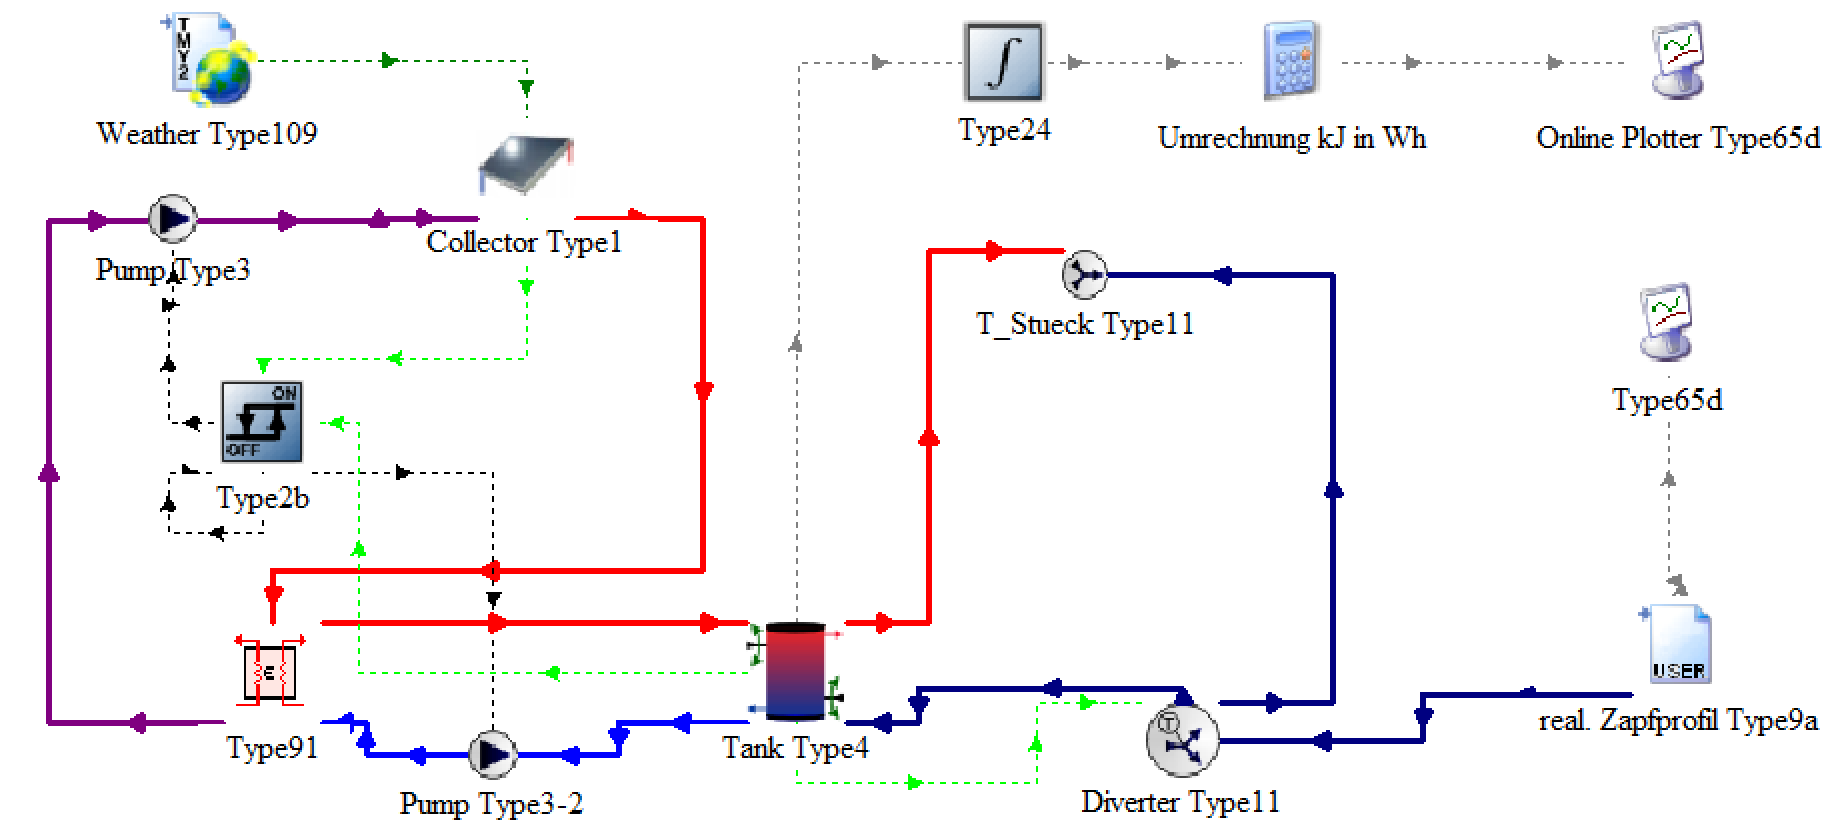
\includegraphics[width=0.8\textwidth]{../DATA/std_deck.png}
	\caption[Grundsystem]{Grundsystem des Decks}
	\label{fig:std_deck}
\end{figure}

Das System basiert auf einem Speicher mit integrierter Nachheizung und externem Wärmeübertrager, an welchen ein Kollektor mit Wetterdaten aus Stuttgart angeschlossen ist. Die Pumpen des Primär- und Sekundärkreislaufes des Wärmeübertragers werden per Temperaturdifferenzregelung angesteuert. Die Kollektortemperatur und die untere Speichertemperatur dienen dem Regler als Vergleichsgrößen. Die Regelung erfolgt als Ein- und Ausschaltsignal. Die Massenströme sind in den Pumpen selbst festgelegt. Ein Verteiler mit Zapfprofil versorgt den Speicher sowie einen Mischer mit Kaltwasser. Der Solare Wärmeeintrag in den Speicher und die Nachheizenergie werden über das Jahr integriert und graphisch ausgegeben.

\subsection{Systemanpassung: Rohrverluste und Kapazitätsströme}
Zur Erweiterung des Systems wird  zwischen dem Kollektor und dem Wärmeübertrager jeweils eine Rohrleitung in Vor- und Rücklauf installiert. Für Die Rohrlänge wurden \SI{9}{\meter} und für den Rohrdurchmesser \SI{2,5}{\centi\meter} angenommen, was zwei bis drei Etagenhöhen zuzüglich horizontaler Abschnitte und Verteilung auf dem Dach entspricht. Die Dicke der Dämmschicht wurde mit \SI{5}{\centi\meter} vorgegeben. Zur Bestimmung des Verlustkoeffizienten werden die Innenmantelfläche des Rohres sowie der UA-Wert benötigt.

\begin{equation}
	\label{eq:Arohr}
	A_{Rohr} = 2*\pi*r*h = 2*\pi*\SI{0,0125}{\meter}*\SI{9}{\meter}=\SI{0,70}{\square\meter}
\end{equation}

\begin{multline}
	\label{eq:UA}
UA = (\frac{1}{2*\pi*l}*(\frac{1}{\alpha_i*r_i}+\sum\frac{ln(\frac{r_{j+1}}{r_j})}{\lambda_j}+\frac{1}{\alpha_a*r_a}))^{-1} = (\frac{1}{2*\pi*\SI{9}{\meter}}\\*(\frac{1}{\SI{1000}{\watt\per\square\meter\per\kelvin}*\SI{0,0125}{\meter}}+\frac{ln(\frac{\SI{16}{\milli\meter}}{\SI{12,5}{\milli\meter}})}{\SI{380}{\watt\per\meter\per\kelvin}}+\frac{ln(\frac{\SI{66}{\milli\meter}}{\SI{16}{\milli\meter}})}{\SI{0,04}{\watt\per\meter\per\kelvin}}\\+\frac{1}{\SI{10}{\watt\per\meter\per\kelvin}*\SI{0,0666}{\meter}}))^{-1}=\SI{1,528}{\watt\per\kelvin}
\end{multline}


\begin{equation}
	\label{eq:U}
	U=\frac{UA}{A_{Rohr}}=\frac{\SI{1,528}{\watt\per\kelvin}}{\SI{0,70}{\square\meter}}=\SI{2,158}{\watt\per\square\meter\per\kelvin}
\end{equation}


Zur Anpassung der Kapazitätsströme wird der Massenstrom der sekundärseitigen Pumpe anhand des Quotienten der Wärmekapazitäten beider Fluide angepasst. Beide Pumpen werden weiterhin mit dem gleichen Regelsignal angesteuert:

\begin{equation}
	\label{eq:dotm}
	\dot m_{2}=\dot m_{1}*\frac{c_{p,1}}{c_{p,2}}
\end{equation}


\subsection{Systemauslegung}
Anhand der Wetterdaten von Stuttgart soll eine solare Deckung von \SI{60}{\percent} für das vorliegende Zapfprofil erzielt werden. Zunächst wurde ein Durchlauf mit den Standardparametern durchgeführt, um den Gesamtwärmebedarf des Systems zu ermitteln. Dieser beträgt jährlich 3240\,kWh. Der solare Jahresertrag $q_{sol}$ wurde mit 450\,kWh pro m\textsuperscript{2} Kollektorfläche geschätzt. Daraus ergibt sich eine Kollektorfläche von

\begin{equation}
	\label{eq:}
	A_{kol}=\frac{Q_{Bedarf}*f_{sol}}{q_{sol}}=\frac{\SI{3240}{\kilo\watt\hour\per\square}*0,6}{\SI{450}{\kilo\watt\hour\per\square\meter}}=\SI{4,32}{\square\meter}
\end{equation}

Bei \SI{50}{\liter\per\square\meter} Speichervolumen entspricht dies einem 200..250\,l Speicher. Für die Simulation wurden beide Größen auf \SI{5}{\square\meter} respektive \SI{250}{\liter} aufgerundet und eine Solare Deckung von

\begin{equation}
	\label{eq:fsolin}
	f_{sol,in} = \frac{Q_{sol}}{Q_{sol}+Q_{aux}} =
\end{equation}
beziehungsweise
\begin{equation}
	\label{eqfsolout:}
	f_{sol,out} = \frac{Q_{sol}-Q_{verl,Sp}}{Q_{TWW+RH}+Q_{Zirk}}=
\end{equation}
unter Berücksichtigung der Verluste erzielt.

\section{Parametervariation}
\subsection{Kaltwasser- und Umgebungstemperatur des Speichers}
Im Rahmen der Parametervariation wurden die Kaltwassertemperatur und die Umgebungstemperatur des Speicherraums in 5-Grad-Schritten von 5..30\si{\celsius} variiert. Insgesamt wurden somit 36 Simulationen durchgeführt. Abbildung \ref{fig:par1} zeigt die erzielte solare Deckung inklusive Verlusten.
\begin{figure}[H]
	\centering
	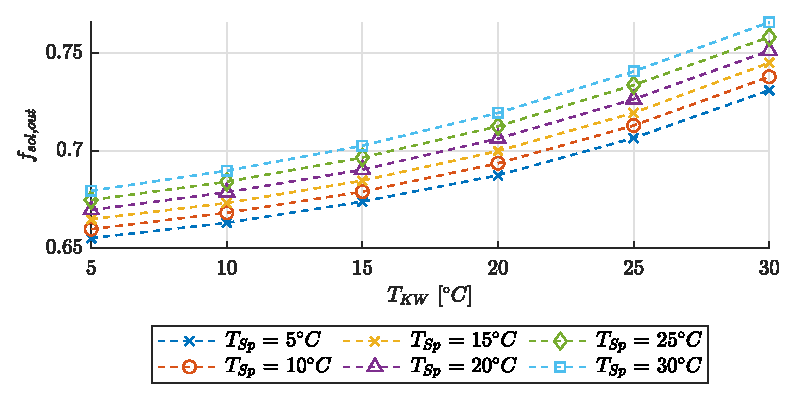
\includegraphics[width=0.8\textwidth]{../DATA/Aufgabe2.2.eps}
	\caption[Parametervariation Kaltwasser und Speicher]{Parametervariation Kaltwasser und Speicher}
	\label{fig:par1}
\end{figure}

Mit zunehmender Raumtemperatur und Kaltwassertemperatur steigt die solare Deckung an. Die Zulauftemperatur hat hierbei den größeren Einfluss von fast 10\,\%, da sie in direkt proportional in den Wärmebedarf einfließt. Die Speicherverluste spielen nur eine untergeordnete Rolle, da der Speicher isoliert ist. Innerhalb der Parametergrenzen unterscheidet sich die solare Deckung um etwa 3\,\%, was jährlich 100\,kWh mehr Solarertrag entspricht.

\subsection{Rohrlänge und Dämmung}
Die Parameter Rohrlänge, Dämmschichtdicke und Wärmeleitfähigkeit wurden jeweils einzeln variiert. Als Grundlage wurden stets die bereits zuvor verwendeten Parameter genutzt und von dort ausgehend immer ein Parameter nach oben und unten variiert.


\begin{figure}[H]
	\centering
	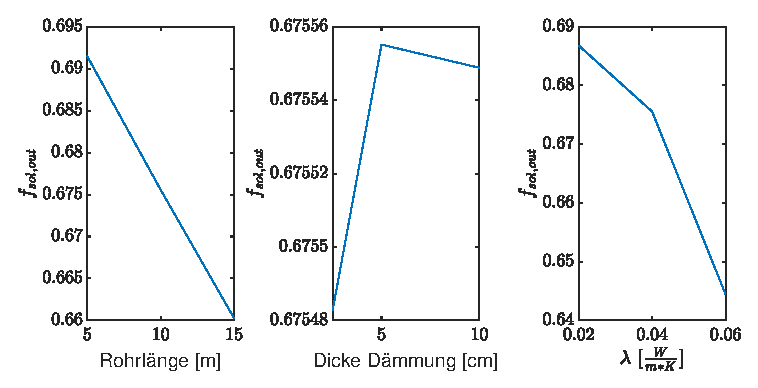
\includegraphics[width=0.8\textwidth]{../DATA/Aufgabe2.3.eps}
	\caption[Parametervariation Dämmung]{Parametervariation Dämmung}
	\label{fig:par2}
\end{figure}

\section{Optimierung der Kollektorparameter}


\section{Parametervariation	}
\subsection{Aufgabenbeschreibung}

Im dritten Teil der Arbeit wurde eine Optimierung der Simulationsparamter mittels Genopt durchgeführt. Für die Optimierung lagen die Messwerte eines Kollektors mit 5 m² Fläche vor. Über einen Zeitraum von 168 Stunden wurden im Viertel-Stunde-Takt die Auslasstemperatur $T_{out}$ Tag wie Nacht gemessen. Zwei Versuche wurden mit jeweils konstanter Zulauftemperatur von 20 °C bzw. 60 °C durchgeführt. Der Volumenstrom betrug während der Messung konstant $20\dfrac{kg}{h*m^2}$.

Ziel der Optimierung war die Anpassung der Kollektorparameter  $\alpha_{0}, \alpha_{1} und \alpha_{2}$ an die Messergebnisse, sodass die Vorlauftemperatur aus dem Kollektormodell mit den Versuchsmesswerten übereinstimmt. 

\begin{equation}
	\label{eq:\eta}
	\eta_{Kol} = \alpha_{0}-\alpha_{1}*\frac{(T_{in}-T_{amb})}{G_{t}}-\alpha_{2}*\frac{(T_{in}-T_{amb})^2}{G_{t}}
\end{equation}

\subsection{Simulationsdurchführung}

Die Optimierung der Parameter erfolgte in zwei Simulationen für $T_{in,1} = 20 °C$ und $T_{in,2} = 60 °C$. Zunächst wurde dem Kollektormodell der gewünschte Volumenstrom und Eingangstemperatur als Inputgröße vorgegeben.
%\newpage
%\input{sections/04_Zusammenfassung_und_Ausblick}

\newpage
%\printbibliography


\end{document}